\renewcommand{\baselinestretch}{2} \small\normalsize
\section{Propagation Statistics}
This chapter describes the propagation factor statistics after numerically propagating over independent random sea surface realizations generated following \cite{frazier_ocean} in a Monte Carlo fashion. First we will discuss the sampling constraints needed to capture the statistics appropriately and then look at the Monte Carlo run setup and provide some example data before finally fitting the PDFs.

\subsection{Sampling Constraints}
The initial set of runs was performed at Ka-Band (35 GHz) and the mean and standard deviation for a 100 run Monte Carlo set are shown in Figure \ref{stat_fig:1}. This data set took over 48 hours to complete running on a laptop and the results were washed out at near range (Figure \ref{stat_fig:1} is clipped at 10 km in near range).

\begin{figure}[H]
  \begin{center}
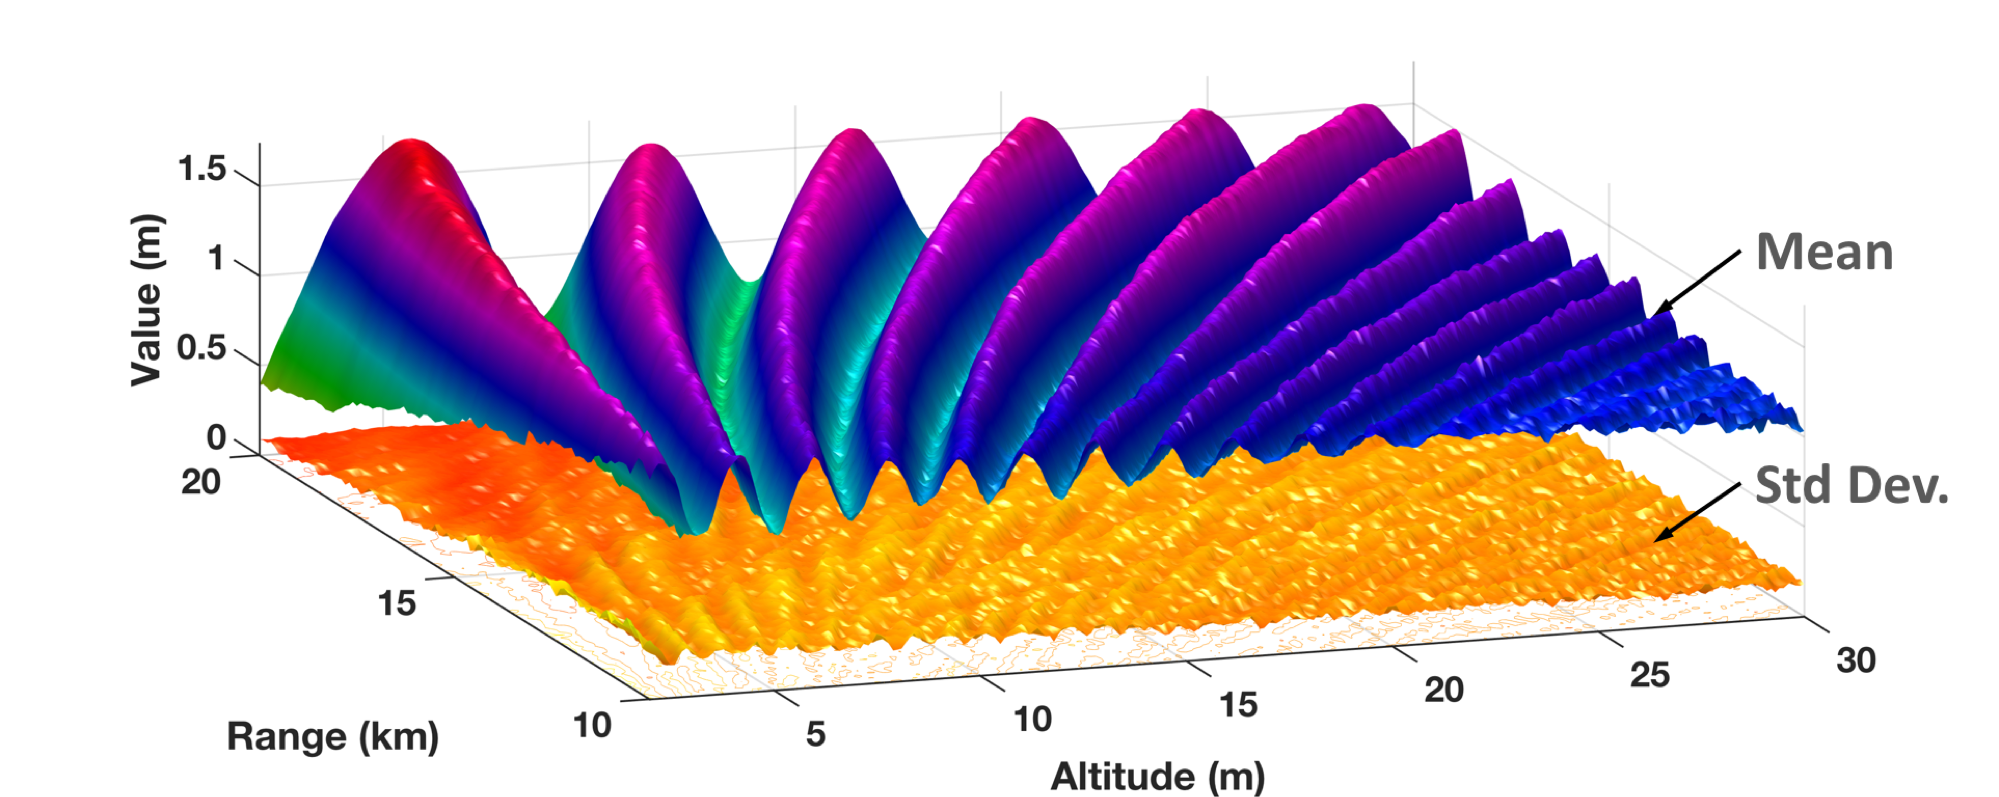
\includegraphics[width=5in]{../media/statistics/ka_band_stats.png}
  \end{center}
  \renewcommand{\baselinestretch}{1} \small\normalsize
  \begin{quote}
    \caption[Ensemble Statistics at Ka-Band with Standard Atmosphere]{Ensemble Statistics at Ka-Band with Standard Atmosphere\label{stat_fig:1}}
  \end{quote}
\end{figure}
\renewcommand{\baselinestretch}{2} \small\normalsize

Figure \ref{stat_fig:2} shows the mean and standard deviation for a 100 run Monte Carlo set at X-band (10 GHz). In this case, the near range results are much cleaner and the data set took less than 6 hours to complete.
\begin{figure}[H]
  \begin{center}
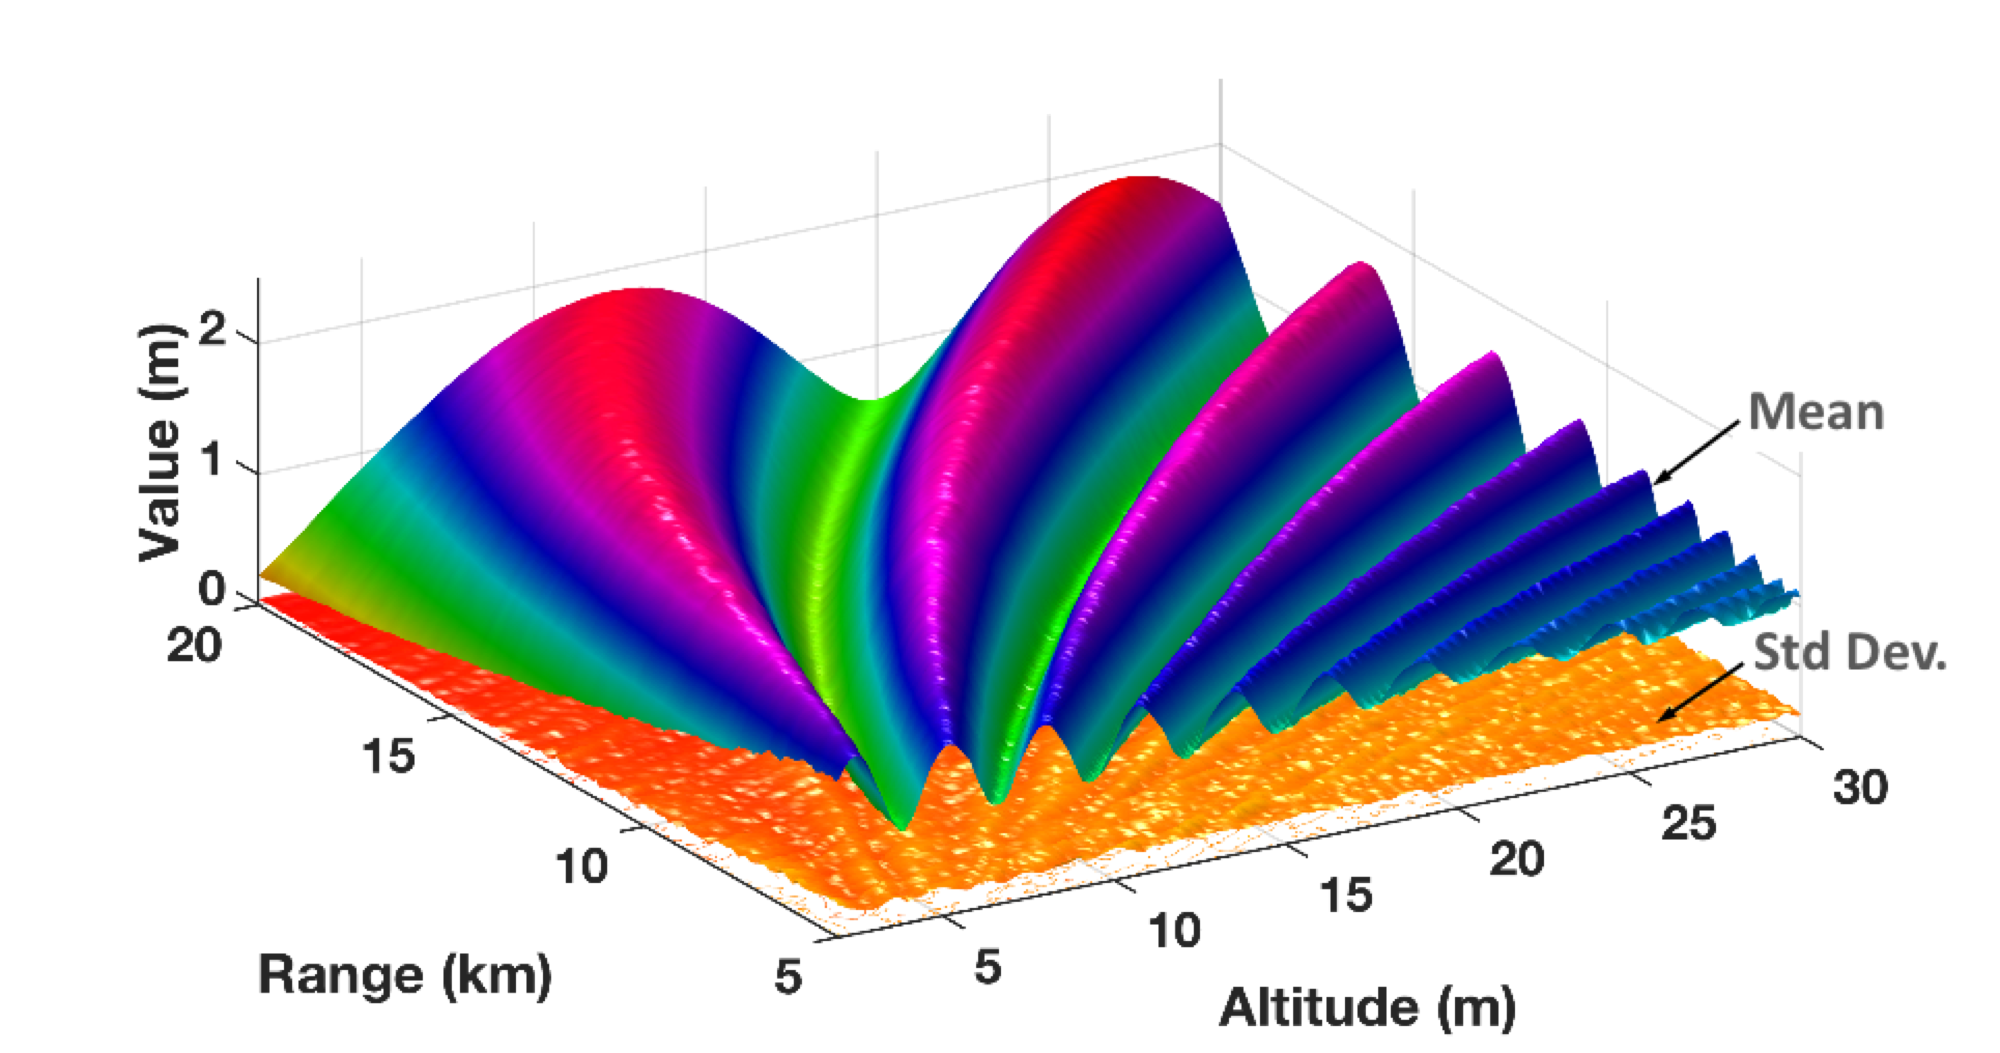
\includegraphics[width=5in]{../media/statistics/x_band_stats.png}
  \end{center}
  \renewcommand{\baselinestretch}{1} \small\normalsize
  \begin{quote}
    \caption[Ensemble Statistics at X-Band with Standard Atmosphere]{Ensemble Statistics at X-Band with Standard Atmosphere\label{stat_fig:2}}
  \end{quote}
\end{figure}
\renewcommand{\baselinestretch}{2} \small\normalsize

These results indicate that spatial sampling constraints from numerical propagation are important for obtaining accurate statistics. This does not mean the numerical propagation method is inaccurate, but that the solution is locally oscillatory so we need finer sampling to correctly capture variations.

To investigate the sampling constraints, we can look at the phase difference between the two primary paths from the propagation factor for the 2 ray model, $F_p = e^{jkL_1} + \Gamma_1e^{jkL_{so}}$. 

\begin{equation}
\begin{gathered}
\Delta\varphi = k\left[ L_1 - L_{so}\right] \\
\Delta\varphi = -\frac{4\pi h_1h_2}{\lambda L}
\label{stat_eq:1}
\end{gathered}
\end{equation}
\renewcommand{\baselinestretch}{2} \small\normalsize

The derivative of the phase difference with respect to range is then

\begin{equation}
\frac{d\Delta\varphi}{dL}=\frac{4\pi h_1h_2}{\lambda L^2}
\label{stat_eq:2}
\end{equation}
\renewcommand{\baselinestretch}{2} \small\normalsize

\noindent This equation can be converted from rad/m to rad/sample by multiplying by the spatial sampling distance in range, $\Delta r$. We can insist that this phase shift per sample be smaller than some pre-determined value to provide adequate sampling. It is often convenient to specify a limit in terms of wavelengths and we can enforce the condition that there must be at least $n$ samples per wavelength of phase difference by letting

\begin{equation}
\frac{4\pi h_1h_2\Delta r}{\lambda L^2} \leq \frac{2\pi \lambda}{n}
\label{stat_eq:3}
\end{equation}

This yields a constraint for the maximum allowable spatial sampling step to ensure $n$ samples per wavelength.
\begin{equation}
\boxed{\Delta r \leq \frac{\lambda^2 L^2}{2nh_1h_2}}
\label{stat_eq:4}
\end{equation}

This equation matches the observation with $n\approx 10$ for the mean values and $n\approx 20$ for the standard deviations. The sampling constraint is shown in Figure \ref{stat_fig:3} for both the 10 and 35 GHz cases, with $n = 20$ and $\Delta r = 0.5$.

\begin{figure}[H]
  \begin{center}
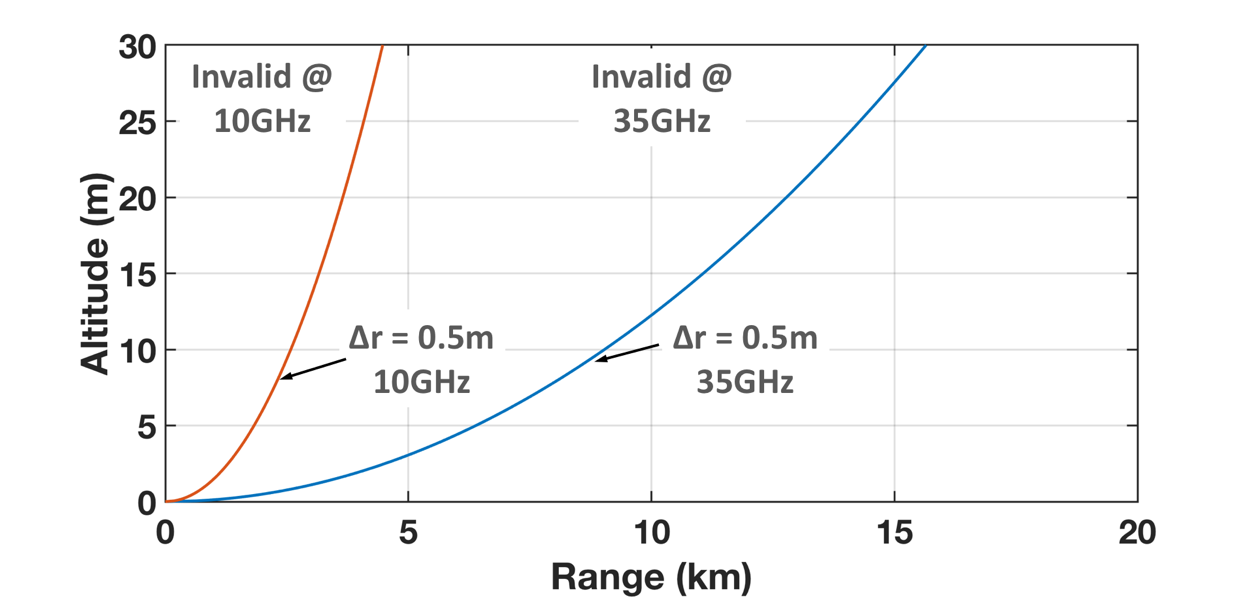
\includegraphics[width=5in]{../media/statistics/sampling_constraint.png}
  \end{center}
  \renewcommand{\baselinestretch}{1} \small\normalsize
  \begin{quote}
    \caption[Sampling Constraints for Statistical Analysis]{Sampling Constraints for Statistical Analysis\label{stat_fig:3}}
  \end{quote}
\end{figure}
\renewcommand{\baselinestretch}{2} \small\normalsize

In order to reduce the sampling constraints and run the Monte Carlo study in a reasonable amount of time, the temporal frequency of interest was changed from 35 GHz to 10 GHz.

\subsection{Monte Carlo Run Methodology}
The data set of propagation factors were generated by creating a random sea surface for a given wind speed and direction, and then numerically propagating using TEMPER. This sequence was repeated for 500 iterations with a different set of random variables for each sea surface.

\subsubsection{Input Parameters}
Table \ref{stat_tab:0} shows the common inputs that were used in all of the Monte Carlo runs.

\begin{table}[H]
  \begin{center}
      \renewcommand{\baselinestretch}{1} \small\normalsize
  \begin{quote}
    \caption[Common Monte Carlo Input Settings]{Common Monte Carlo Input Settings\label{stat_tab:1}}
  \end{quote}
  \begin{tabular} {|c | c |}
    \hline
  \bf{Parameter} & \bf{Value} \\ \hline
  Frequency & 10 GHz \\ \hline
  Antenna Pattern & Sinc \\ \hline
  Antenna Beamwidth & $8^{\circ}$  \\ \hline
  Polarization & Vertical \\ \hline
  Transmitter Height & 30 m \\ \hline
  Maximum Range & 20 km \\ \hline
  Range Step & 0.5 m  \\ \hline
  Maximum Altitude & 30 m \\ \hline
  Earth Model & Spherical \\ \hline
  Inverse Age Parameter & 0.84 (fully developed) \\ \hline
  Initial Seed & 561894\\ \hline
  Number of Runs & 500\\ \hline
\end{tabular}
\end{center}
\end{table}
\renewcommand{\baselinestretch}{2} \small\normalsize

The parameterizations resulted in 26 total data sets to capture the effect of wind speed (from 2 m/s to 15 m/s at $0^{\circ}$ wind direction), wind direction ($90^{\circ}$ to $0^{\circ}$ at 10 m/s wind speed), and refractive index profile (standard atmosphere and a 20 m duct). Table \ref{stat_tab:1} shows the primary run matrix with the various parameterizations. 

\begin{table}[H]
  \begin{center}
      \renewcommand{\baselinestretch}{1} \small\normalsize
  \begin{quote}
    \caption[Monte Carlo Propagation Run Matrix]{Monte Carlo Propagation Run Matrix\label{stat_tab:0}}
  \end{quote}
  \begin{tabular} {|c | c | c| c |}
    \hline
  \bf{Dataset ID} & \bf{Wind Speed} & \bf{Wind Direction} & \bf{Refractivity}  \\ \hline
  1 & 2 m/s & $0^{\circ}$ & Standard Atmosphere \\ \hline
  2 & 3 m/s & $0^{\circ}$ & Standard Atmosphere \\ \hline
  3 & 4 m/s & $0^{\circ}$ & Standard Atmosphere \\ \hline
  4 & 5 m/s & $0^{\circ}$ & Standard Atmosphere \\ \hline
  5 & 8 m/s & $0^{\circ}$ & Standard Atmosphere \\ \hline
  6 & 10 m/s & $0^{\circ}$ & Standard Atmosphere \\ \hline
  7 & 12 m/s & $0^{\circ}$ & Standard Atmosphere \\ \hline
  8 & 15 m/s & $0^{\circ}$ & Standard Atmosphere \\ \hline
  9 & 10 m/s & $18^{\circ}$ & Standard Atmosphere \\ \hline
  10 & 10 m/s & $36^{\circ}$ & Standard Atmosphere \\ \hline
  11 & 10 m/s & $54^{\circ}$ &  Standard Atmosphere\\ \hline
  12 & 10 m/s & $72^{\circ}$ &  Standard Atmosphere \\ \hline
  13 & 10 m/s & $90^{\circ}$ &  Standard Atmosphere \\ \hline
  14 & 2 m/s & $0^{\circ}$ & 20 m Duct \\ \hline
  15 & 3 m/s & $0^{\circ}$ & 20 m Duct \\ \hline
  16 & 4 m/s & $0^{\circ}$ & 20 m Duct \\ \hline
  17 & 5 m/s & $0^{\circ}$ & 20 m Duct \\ \hline
  18 & 6 m/s & $0^{\circ}$ & 20 m Duct \\ \hline
  19 & 10 m/s & $0^{\circ}$ & 20 m Duct \\ \hline
  20 & 12 m/s & $0^{\circ}$ & 20 m Duct \\ \hline
  21 & 15 m/s & $0^{\circ}$ & 20 m Duct \\ \hline
  22 & 10 m/s & $18^{\circ}$ & 20 m Duct \\ \hline
  23 & 10 m/s & $36^{\circ}$ & 20 m Duct \\ \hline
  24 & 10 m/s & $54^{\circ}$ & 20 m Duct \\ \hline
  25 & 10 m/s & $72^{\circ}$ & 20 m Duct \\ \hline
  26 & 10 m/s & $90^{\circ}$ & 20 m Duct \\ \hline
\end{tabular}
\end{center}
\end{table}
\renewcommand{\baselinestretch}{2} \small\normalsize

\subsection{Example Results}
Figure \ref{stat_fig:1a} and Figure \ref{stat_fig:1b} show example propagation factors from two specific sea surface realizations from dataset $6$ (10 m/s, $0^{\circ}$, standard atmosphere).

\begin{figure}[H]
  \begin{center}
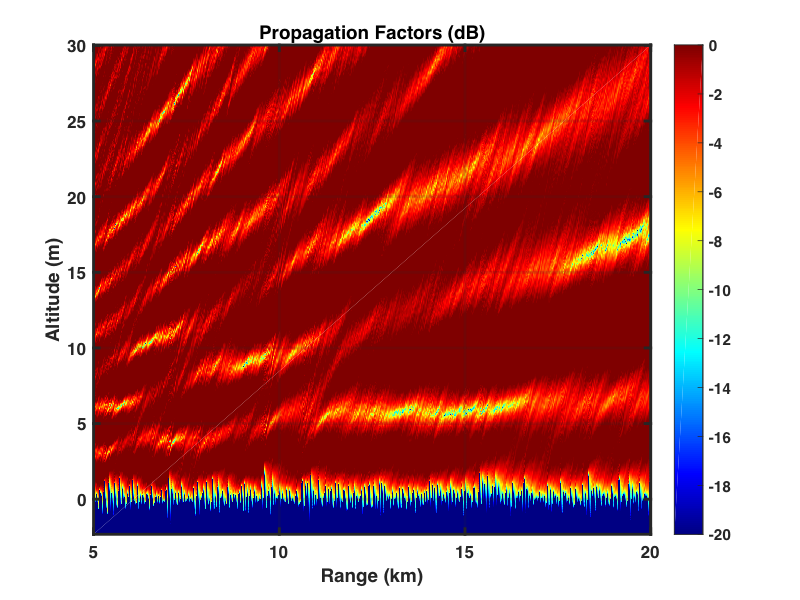
\includegraphics[width=4in]{../media/statistics/pf_1.png}
  \end{center}
  \renewcommand{\baselinestretch}{1} \small\normalsize
  \begin{quote}
    \caption[Example Propagation Factor Realization]{Example Propagation Factor Realization\label{stat_fig:1a}}
  \end{quote}
\end{figure}
\renewcommand{\baselinestretch}{2} \small\normalsize

\begin{figure}[H]
  \begin{center}
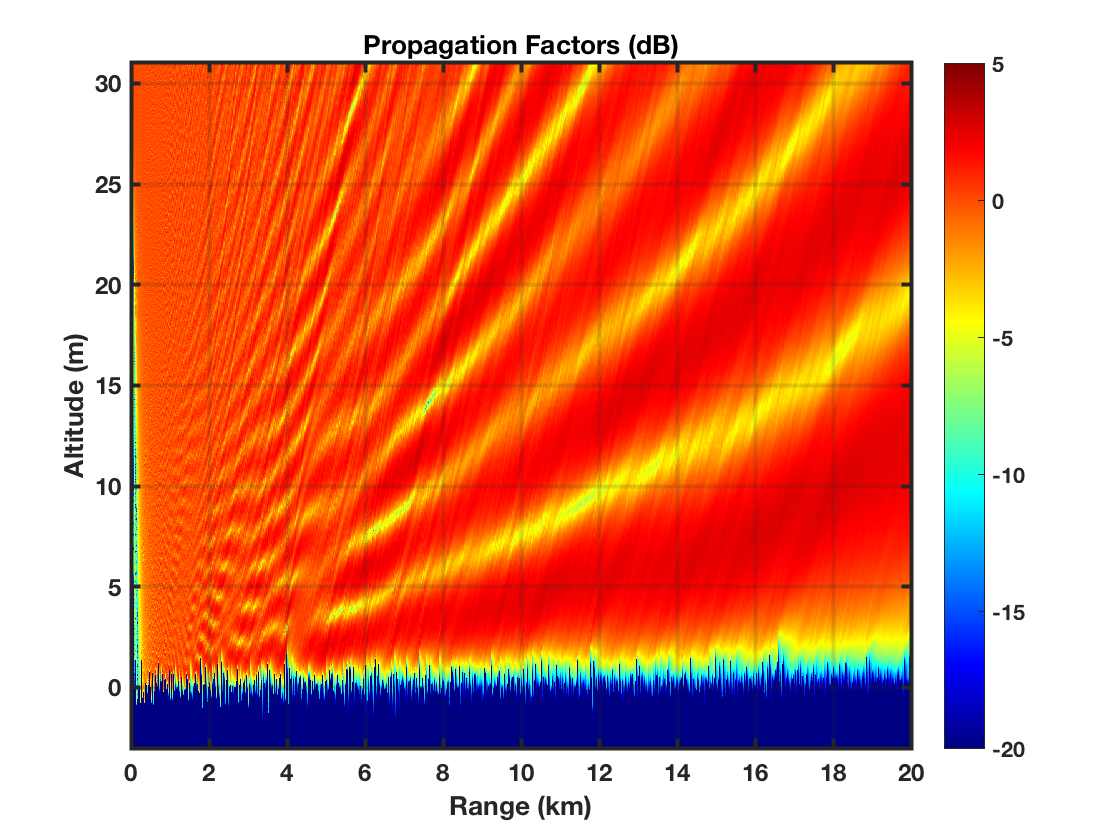
\includegraphics[width=4in]{../media/statistics/pf_2.png}
  \end{center}
  \renewcommand{\baselinestretch}{1} \small\normalsize
  \begin{quote}
    \caption[Example Propagation Factor Realization]{Example Propagation Factor Realization\label{stat_fig:1b}}
  \end{quote}
\end{figure}
\renewcommand{\baselinestretch}{2} \small\normalsize

\subsection{General Monte Carlo Results}
The mean and standard deviation with a 5 m/s wind speed and a $0^\circ$ wind direction are shown in Figure \ref{stat_fig:1zz} for standard atmosphere, and in Figure \ref{stat_fig:1zzz} for a 20 m duct.

\begin{figure}[H]
  \begin{center}
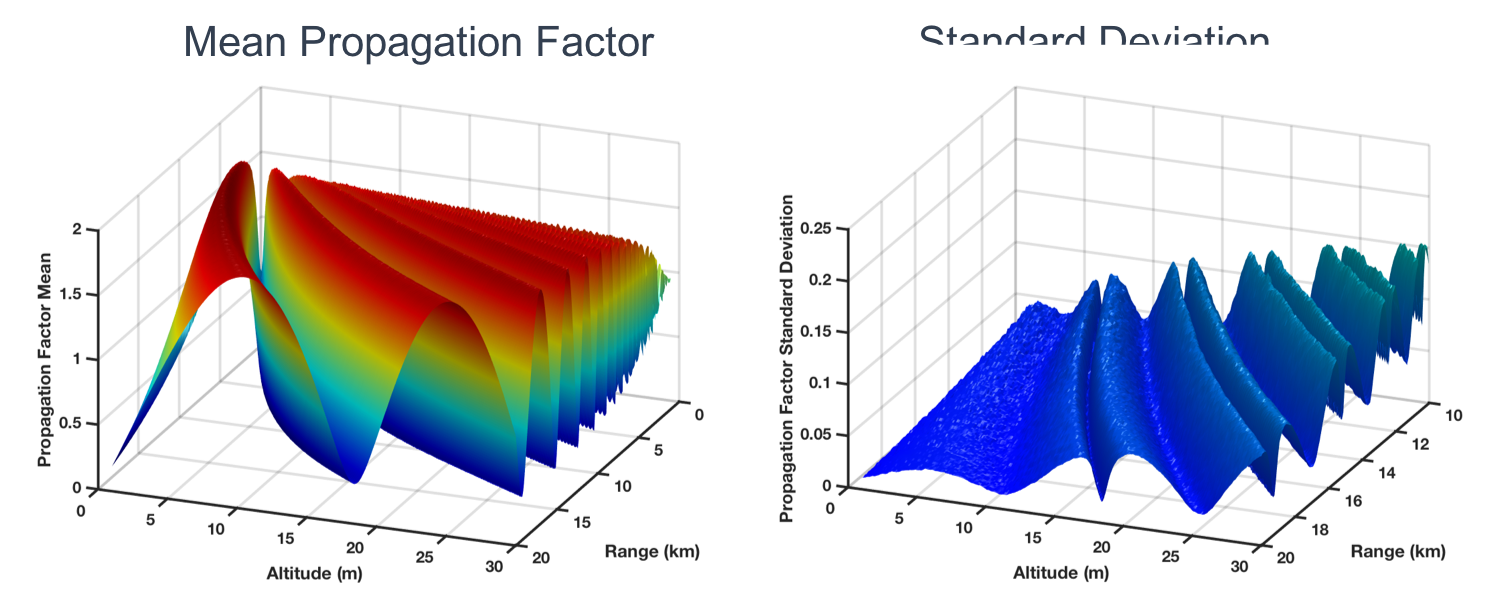
\includegraphics[width=5.5in]{../media/multistatic/std_atmos_results.png}
  \end{center}
  \renewcommand{\baselinestretch}{1} \small\normalsize
  \begin{quote}
    \caption[Standard Atmosphere Statistics at 5 m/s and $0^{\circ}$ Wind]{Standard Atmosphere Statistics at 5 m/s and $0^{\circ}$ Wind\label{stat_fig:1zz}}
  \end{quote}
\end{figure}
\renewcommand{\baselinestretch}{2} \small\normalsize

\begin{figure}[H]
  \begin{center}
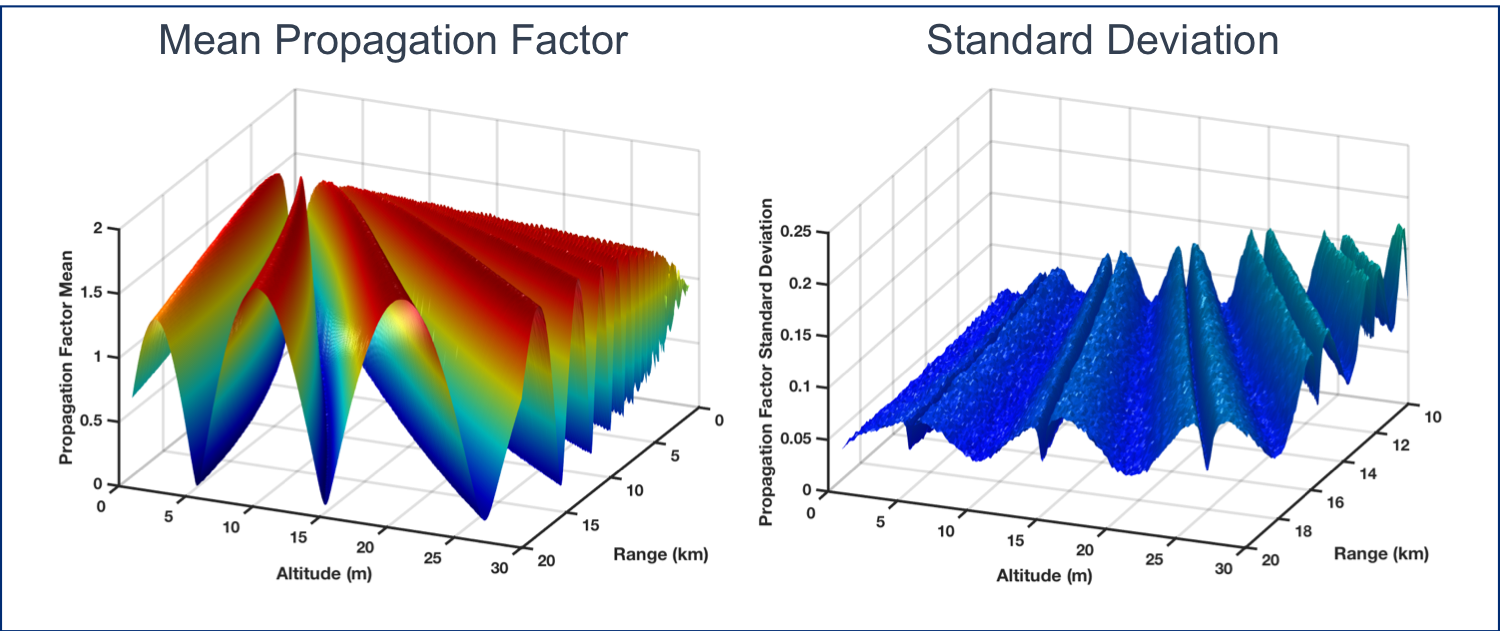
\includegraphics[width=5.5in]{../media/multistatic/duct_results.png}
  \end{center}
  \renewcommand{\baselinestretch}{1} \small\normalsize
  \begin{quote}
    \caption[20 m Duct Statistics at 5 m/s and $0^{\circ}$ Wind]{20 m Duct Statistics at 5 m/s and $0^{\circ}$ Wind\label{stat_fig:1zzz}}
  \end{quote}
\end{figure}
\renewcommand{\baselinestretch}{2} \small\normalsize

In both of these cases, we see that the standard deviation has deep nulls that are co-aligned with nulls in the mean and shallower nulls that are co-aligned with peaks in the mean. These results make sense if we think of propagation of a bundle of rays; at the peaks and nulls in the mean, the rays are all either strongly coherent (peak) or strongly anti-coherent (null). At these extremes, there is little phase variation between the waves and less room for variation in received power. This result also indicates that the standard deviation oscillates at twice the rate of the mean value. 

\subsection{Diffractive Phase Shift}
Figure \ref{stat_fig:2zz} shows the mean propagation factor vs. altitude at a constant range (20 km) for various wind speeds and Figure \ref{stat_fig:2zzz} shows the mean propagation factor vs. altitude at a constant range (20 km) for various wind direction angles. These plots demonstrate there is a diffractive phase shift incurred when propagating over a numerical surface instead of a flat surface with the Miller-Brown approximation.

\begin{figure}[H]
  \begin{center}
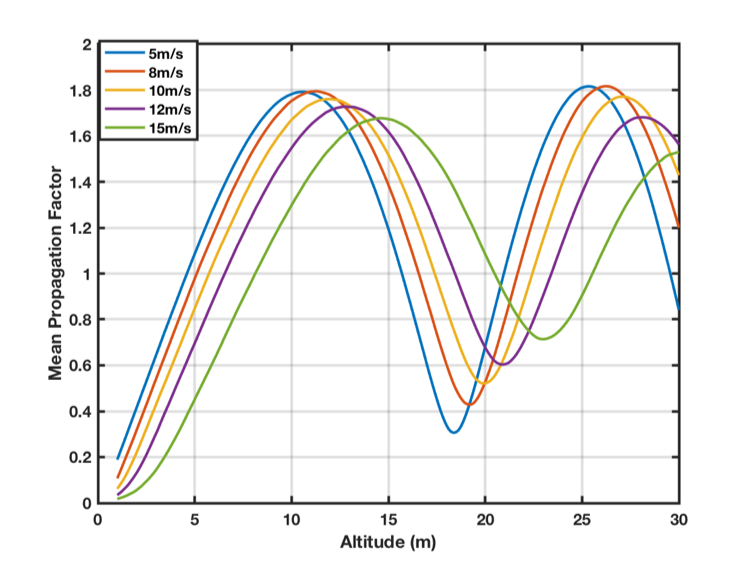
\includegraphics[width=4in]{../media/statistics/phase_shift_wind_speed.png}
  \end{center}
  \renewcommand{\baselinestretch}{1} \small\normalsize
  \begin{quote}
    \caption[Phase Shift at Constant Range due to Wind Speed]{Phase Shift at Constant Range due to Wind Speed\label{stat_fig:2zz}}
  \end{quote}
\end{figure}
\renewcommand{\baselinestretch}{2} \small\normalsize

As shown in Figure \ref{stat_fig:2zz}, increasing the wind speed reduces the amplitude of the mean propagation factor and shifts the phase of the multipath peaks and nulls upward in altitude. The amplitude reduction is expected because higher wind speeds create sea surfaces with more energy which in turn means less RF energy is reflected in the forward direction.

\begin{figure}[H]
  \begin{center}
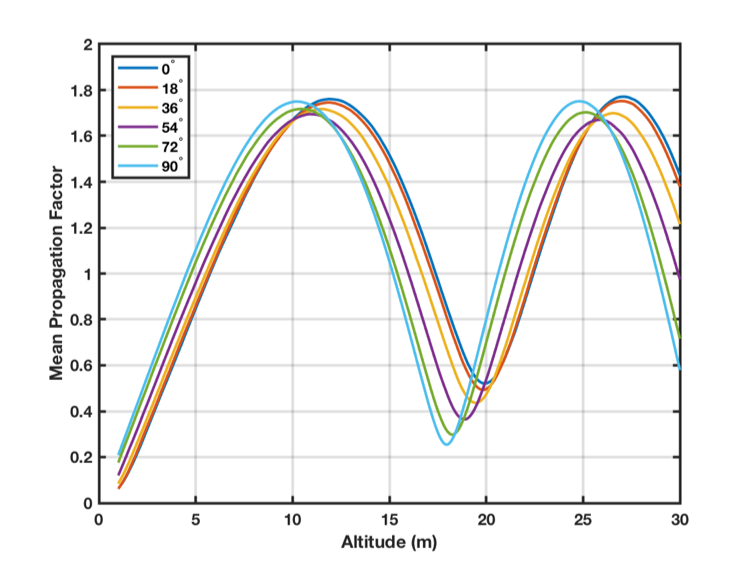
\includegraphics[width=4in]{../media/statistics/phase_shift_wind_direction.png}
  \end{center}
  \renewcommand{\baselinestretch}{1} \small\normalsize
  \begin{quote}
    \caption[Phase Shift at Constant Range due to Wind Direction]{Phase Shift at Constant Range due to Wind Direction\label{stat_fig:2zzz}}
  \end{quote}
\end{figure}
\renewcommand{\baselinestretch}{2} \small\normalsize

As shown in Figure \ref{stat_fig:2zzz}, decreasing the wind direction also shifts the phase of the multipath peaks and nulls upward. In this case, the amplitude does not monotonically decrease because changing the wind direction actually changes the power spectrum surface \cite{frazier_ocean} rather than simply affecting the overall amplitude.

\subsection{PDF Fitting Results}
Propagation over the open ocean should result in a system with fairly high losses, so we expect the PDFs to be normally distributed \cite{yeh_first_principles} \cite{yeh_fading}. 

\subsubsection{Example Fitting Metrics}
Figure \ref{stat_fig:4} shows the propagation factor fit at constant range (20 km) at 10 m and 30 m altitude to demonstrate fitting around both a multipath peak and a multipath null. The standard deviation in both cases shown is identical ($\sigma = 0.176$) and in general is very similar for fits made at a constant range but different altitudes.

\begin{figure}[H]
  \begin{center}
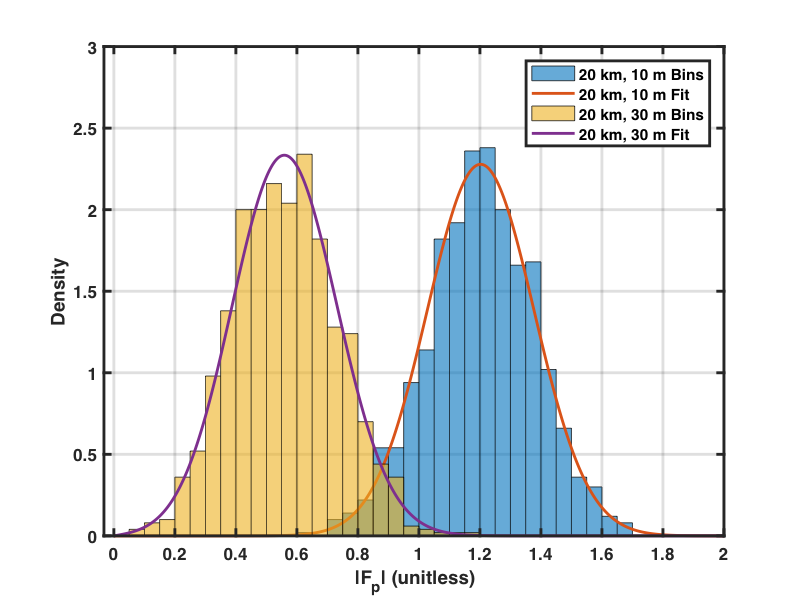
\includegraphics[width=4in]{../media/statistics/constant_range_fit.png}
  \end{center}
  \renewcommand{\baselinestretch}{1} \small\normalsize
  \begin{quote}
    \caption[PDF Fitting at Constant Range]{PDF Fitting at Constant Range\label{stat_fig:4}}
  \end{quote}
\end{figure}
\renewcommand{\baselinestretch}{2} \small\normalsize

Figure \ref{stat_fig:5} shows the propagation factor fit at constant altitude (10 m) at 10 km and 15 km range, again to demonstrate fitting around both a multipath peak and a multipath null. The standard deviation is no longer the same ($\sigma_{10} = 0.223$ while $\sigma_{15} = 0.188$). In general, the standard deviation is not similar for fits made at a constant altitude but different ranges. This indicates range has a stronger impact than altitude.

\begin{figure}[H]
  \begin{center}
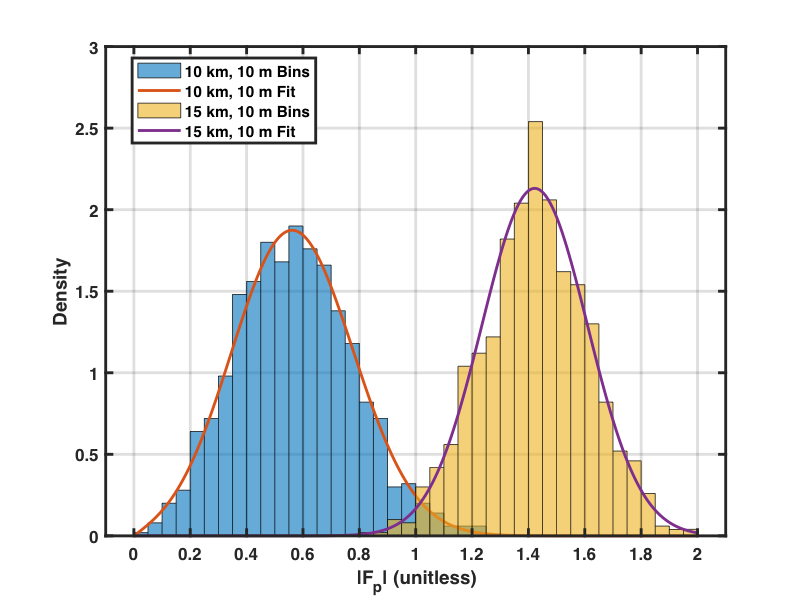
\includegraphics[width=4in]{../media/statistics/constant_altitude_fit.png}
  \end{center}
  \renewcommand{\baselinestretch}{1} \small\normalsize
  \begin{quote}
    \caption[PDF Fitting at Constant Altitude]{PDF Fitting at Constant Altitude\label{stat_fig:5}}
  \end{quote}
\end{figure}
\renewcommand{\baselinestretch}{2} \small\normalsize

\subsection{Loss Parameter Estimation}
As shown in \cite{yeh_fading}, the relationship between the standard deviation, $\sigma$, of the PDF and the loss parameter, $\alpha$, that describes the RMT result is given by

\begin{equation}
\alpha = \frac{1}{\pi\sigma^2}
\end{equation}
\renewcommand{\baselinestretch}{2} \small\normalsize

With this relationship, we can use RMT to match the signal fluctuations around a predetermined average propagation factor.

From \cite{frazier_green}, we can express the phase difference between the primary and the reflected ray as

\begin{equation}
\Delta\phi = 2k\frac{h_1h_2}{L}
\end{equation}
\renewcommand{\baselinestretch}{2} \small\normalsize

Using the observation that the standard deviation oscillates at twice the rate of the mean value, we can break the standard deviation, $\sigma$, into an oscillatory term, $\sigma_s$, and an envelope term $\sigma_d$ so that $\sigma = \sigma_s \sigma_d$. The mean value oscillates relative to $Re\{\exp\left[j\Delta\phi\right]\} = \cos\left(\Delta\phi\right)$. Because the standard deviation must be out of phase with the mean, $\sigma_s$ can be approximated as:

\begin{equation}
\sigma_s = \sin^2\left(2k\frac{h_1h_2}{L}\right)
\end{equation}
\renewcommand{\baselinestretch}{2} \small\normalsize

For a 1-d system, the loss parameter can be approximated as $a \approx kL/Q$, where $Q$ is the quality factor of a given cavity. $Q$ is defined as \cite{pozar_microwave}

\begin{equation}
Q = \omega_0\frac{\text{Energy Stored}}{\text{Power Lost}}
\end{equation}
\renewcommand{\baselinestretch}{2} \small\normalsize

For sufficiently shallow grazing angles there is little backscatter for clutter and we can assume all the energy is either absorbed into the ocean or scattered forward towards the target. Because we are working with propagation factors, we can normalize the transmitted power and approximate an effective quality factor as

\begin{equation}
Q \approx \omega_o\frac{1-\Gamma_t}{\Gamma_t^2}
\end{equation}
\renewcommand{\baselinestretch}{2} \small\normalsize

Here, $\Gamma_t$ is the total reflection coefficient as described in Section \ref{section_reflection_coefficient}, which is dependent on the grazing angle and the RMS ocean wave height, $\sigma_h$.

RMT predicts that the voltage fluctuations will be normally distributed with standard deviation given by $\sigma = \sqrt{(\pi \alpha)^{-1}}$. Since we are looking at fluctuations in power, this standard deviation in voltage will be the variance in power so that

\begin{equation}
\sigma_d = \sqrt{\sigma} = \left( \frac{1}{\pi\alpha} \right)^{1/4}
\end{equation}
\renewcommand{\baselinestretch}{2} \small\normalsize

This assumes that the entire path length, $L$, contributes, so we need to add a scale factor that is the ratio of the region over which the reflected energy is not negligible, $\tilde{x}$ to the total down range distance, $L$. With this scale factor, the envelope term becomes:

\begin{equation}
\sigma_d \approx \frac{1}{4} \left(\frac{1}{\pi \alpha}\right)^{1/4}\left(\frac{\tilde{x}}{L}\right)
\end{equation}
\renewcommand{\baselinestretch}{2} \small\normalsize

\noindent From \cite{frazier_green}, we can express $\tilde{x}$ as:

\begin{equation}
\tilde{x} = \sqrt{\frac{2}{kL_0''}}
\end{equation}
\renewcommand{\baselinestretch}{2} \small\normalsize

\noindent Where $L_0''$ is given as:
\begin{equation}
L_0''=\frac{(h_1+h_2)^4}{h_1h_2L^3} 
\end{equation}
\renewcommand{\baselinestretch}{2} \small\normalsize

\noindent The predicted propagation factor standard deviation is then:
\begin{equation}
\sigma = \sin^2\left(2k\frac{h_1h_2}{L}\right) \frac{1}{4}\left(\frac{\omega_0(1-\Gamma_t)}{\pi kL\Gamma_t^2}\right)^{1/4}\left(\frac{\tilde{x}}{L}\right)
\label{stat_eq:zzz}
\end{equation}
\renewcommand{\baselinestretch}{2} \small\normalsize

Figure \ref{stat_fig:a1} compares the predicted result with the numerical results for 10 mps wind speed at two different wind directions (0 $^{\circ}$ and 36$^{\circ}$). The target point in both cases is at 20 m in altitude.

\begin{figure}[H]
  \begin{center}
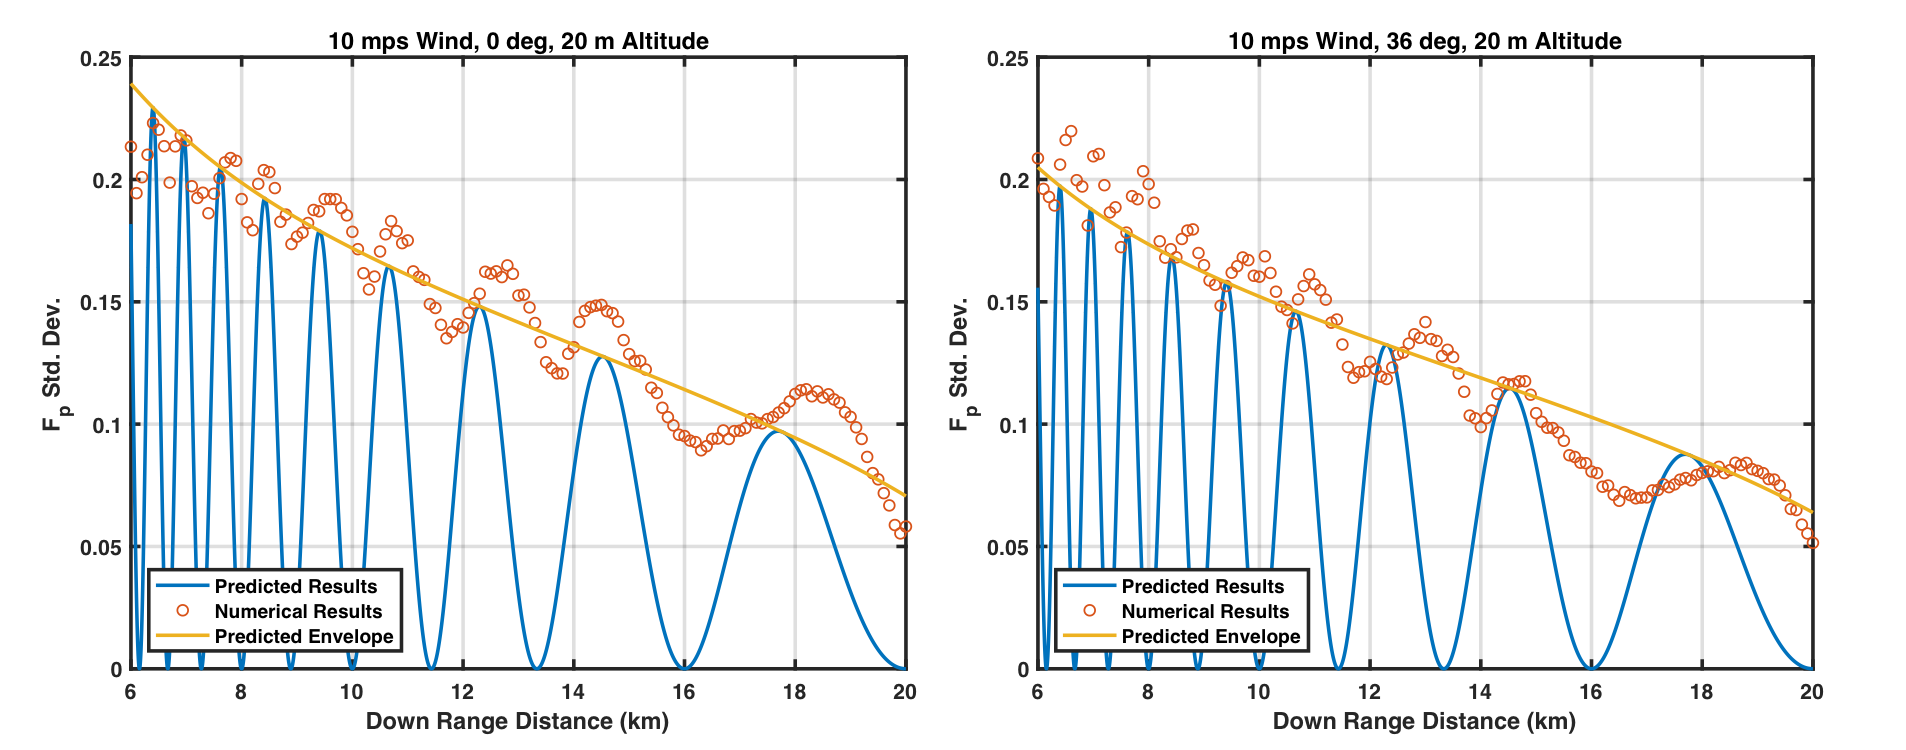
\includegraphics[width=6in]{../media/statistics/predicted_results_wind_direction.png}
  \end{center}
  \renewcommand{\baselinestretch}{1} \small\normalsize
  \begin{quote}
    \caption[$F_p$ Standard Deviation Comparison vs. Wind Direction]{$F_p$ Standard Deviation Comparison vs. Wind Direction\label{stat_fig:a1}}
  \end{quote}
\end{figure}
\renewcommand{\baselinestretch}{2} \small\normalsize

Figure \ref{stat_fig:a1} compares the predicted result with the numerical results directly down range (0$^{\circ}$ wind direction) at two different wind speeds (8 mps and 12 mps). Again, the target point in both cases is at 20 m in altitude.

\begin{figure}[H]
  \begin{center}
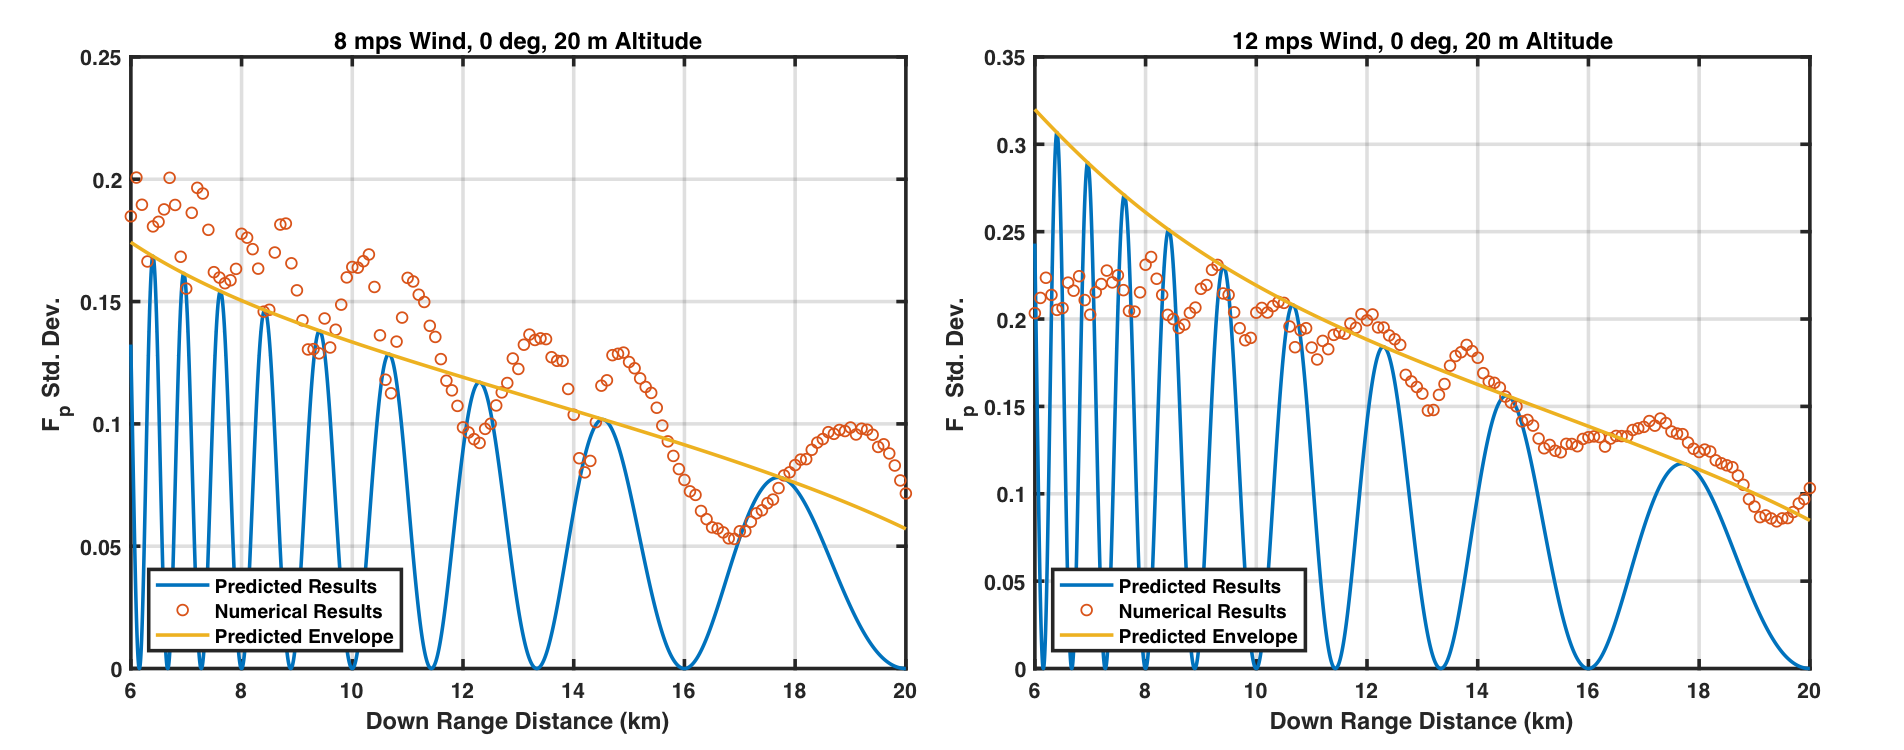
\includegraphics[width=6in]{../media/statistics/predicted_results_wind_speed.png}
  \end{center}
  \renewcommand{\baselinestretch}{1} \small\normalsize
  \begin{quote}
    \caption[$F_p$ Standard Deviation Comparison vs. Wind Speed]{$F_p$ Standard Deviation Comparison vs. Wind Speed\label{stat_fig:a2}}
  \end{quote}
\end{figure}
\renewcommand{\baselinestretch}{2} \small\normalsize 

In both Figure \ref{stat_fig:a1} and Figure \ref{stat_fig:a2}, the envelope term is a good match for the standard deviation when the assumption of shallow grazing angles is valid. As the wind speed increases, this assumption becomes tighter and indicates deviations from the model at short ranges. The location of the peaks and nulls do not line up because the predicted results do not include any corrections for the phase shift. 

Equation \ref {stat_eq:zzz} provides a reasonable approximation for the propagation factor standard deviations shown in Figure \ref{stat_fig:1zz} and Figure \ref{stat_fig:1zzz} but does not include the diffractive phase shift. Using this equation allows us to include propagation factor statistics around a single TEMPER baseline run rather than requiring many iterations. More work is needed to verify this approach over a wider range of conditions and determine the limitations for various geometries.